The given curve,
\begin{align}
    \vec{x}^T\vec{x}-2\myvec{1&0}\vec{x}-3=0
\end{align}
has parameters
\begin{align}
    \vec{V}=\myvec{1&0\\0&1}=\vec{V}^{-1}, \vec{u}=\myvec{1\\0}, f=0
\end{align}
% \begin{align}
%     \because |\vec{V}|>0
% \end{align}
Hence, the given curve is a circle. The point of contact for the tangent is
\begin{align}
    \vec{q}=\vec{V}^{-1}(\kappa \vec{n}-\vec{u})
    \label{eq.1}
\end{align}
where,
\begin{align}
    \kappa=\pm\sqrt{\frac{\vec{u}^T\vec{V}^{-1}\vec{u}-f}{\vec{n}^T\vec{V}^{-1}\vec{n}}} 
\end{align}
For the tangents parallel to x-axis, the direction and normal vectors are 
\begin{align}
    \vec{m}=\myvec{1\\0}, \vec{n}=\myvec{0\\1}\end{align}
    \begin{align}
        \kappa&=\pm\sqrt{\frac{\vec{u}^T\vec{V}^{-1}\vec{u}-f}{\vec{n}^T\vec{V}^{-1}\vec{n}}}\\
        &=\pm2
    \end{align}
By substituting $\kappa, \vec{n}, \vec{V}^{-1}$ in \eqref{eq.1}
\begin{align}
    \vec{q}&=\vec{V}^{-1}(\kappa \vec{n}-\vec{u})\\
    &=\myvec{-1\\\pm2}
\end{align}

\begin{figure}[h]
\centering
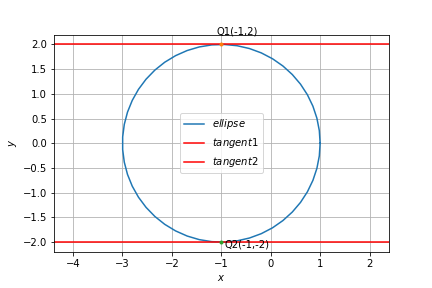
\includegraphics[width=\columnwidth]{solutions/sep/2/4/Figures/ellipse.1.png}
\caption{Ellipse with tangents parallel to x axis at points $\vec{q}=\myvec{-1\\\pm2}$}
\label{Fig 1.1}

\end{figure}

